\documentclass[addpoints,12pt]{exam}
\usepackage{amsmath}
\usepackage{amsthm}
\usepackage{amsfonts}
\usepackage{systeme}
\usepackage{graphicx}
\usepackage{caption}
\usepackage{xfrac}
\usepackage{physics}
\usepackage{microtype}
\usepackage{eulervm}
%\usepackage[framemethod=tikz]{mdframed}
\usepackage{thmtools}
\usepackage{etoolbox}
%\usepackage{fouriernc}

\pagestyle{headandfoot}
\runningfootrule
\firstpageheadrule
\runningheadrule

\newcommand{\class}{Math 0098}
\newcommand{\sem}{2201}
\newcommand{\due}{}
\newcommand{\sect}{8.2}
\newcommand{\topic}{Graphs of Functions}

\firstpageheader{\class}{\sect - \topic}{}
\runningheader{\class}{\sect - \topic}{}
\firstpagefooter{\class}{}{Page \thepage\ of \numpages}
\runningfooter{\class}{}{Page \thepage\ of \numpages}

\newif\ifprintselected
\printselectedtrue
%\printselectedfalse

\newenvironment{select}
{\ifprintselected
	\printanswers
	\fi
}
{}

\theoremstyle{definition}
\newtheorem{theorem}{Theorem}
\newtheorem{example}{Example}[subsection]
%\newtheorem{definition}{Definition}
\newtheorem{definition}{Definition}[subsection]
%\newmdtheoremenv{example}{Example}[subsection]
\AtBeginEnvironment{defn}{\begin{minipage}{\textwidth}}
\AtEndEnvironment{defn}{\end{minipage}}
%\AtBeginEnvironment{example}{\begin{minipage}{\textwidth}}
%\AtEndEnvironment{example}{\end{minipage}}
\newcommand{\iu}{{i\mkern1mu}}

\setlength{\gridsize}{5mm}
\setlength{\gridlinewidth}{0.1pt}

\printanswers
\DeclareMathSizes{12}{12}{12}{12}

\begin{document}
\setcounter{section}{8}
\setcounter{subsection}{2}

In Algebra 1, we graphed linear equations - equations in the form of $y = mx + b$ - by using the slope and the $y$-intercept. We also graphed quadratic equations by making a table of values. When we graph \emph{functions}, we use the same process.

\vspace{.25in}

We are able to determine if a graph is the graph of a function if it passes the \emph{vertical line test}.

\vspace{.25in}
\begin{definition}[Vertical Line Test]
If any vertical line intersects a graph in more than one point, the graph does not represent $y$ as a function of $x$ ($y(x)$).
\end{definition}

\begin{example}
Use the vertical line test to determine whether or not each of the following graphs represents a function. 

\begin{minipage}{.33\textwidth}
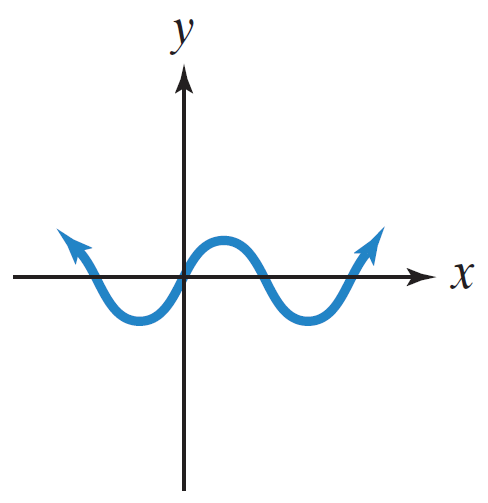
\includegraphics[scale=.4]{images/vert_line_test_01}
\end{minipage}%
\begin{minipage}{.33\textwidth}
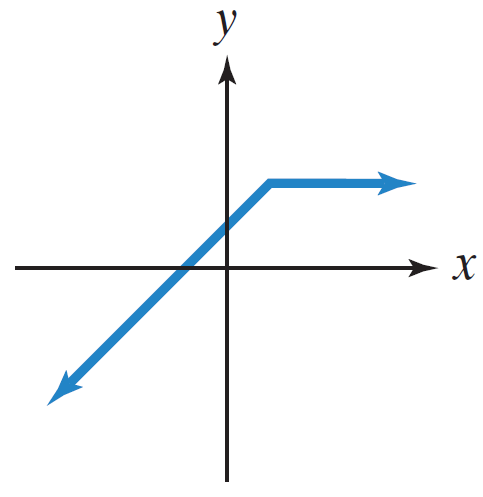
\includegraphics[scale=.4]{images/vert_line_test_02}
\end{minipage}%
\begin{minipage}{.33\textwidth}
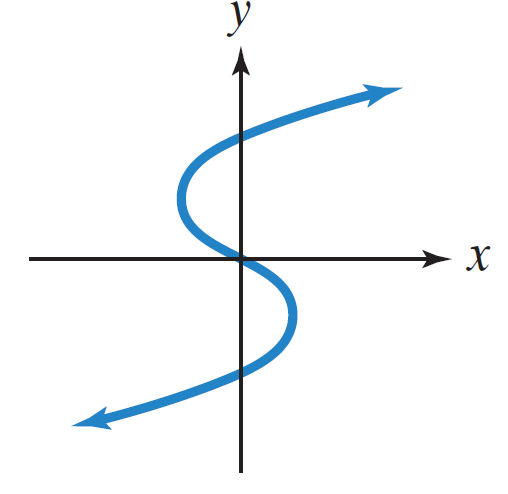
\includegraphics[scale=.4]{images/vert_line_test_03}
\end{minipage}%
\end{example}

\vspace{.5in}

\subsubsection*{Interval Notation}

An \emph{interval} of numbers is a portion of the number line between some two values. We can represent an interval in \emph{set-builder notation}, \emph{inequality notation} and as a graph on a number line. Remember that with intervals, parentheses, (), show that a value is not included and that square brackets, [], show that values are included.

\newpage

\begin{figure}[h]
\centering
\begin{tabular}{c | c | c}
\textbf{Interval Notation} & \textbf{Set-Builder Notation} & \textbf{Graph}\\\hline
& &$\;\;\;\;\;\;\;\;\;\;\;\;\;\;\;\;\;\;\;\;\;\;\;\;\;\;\;\;\;\;\;\;\;\;\;$\\
& &\\
$(a,b)$ & & \\ 
& &\\\hline
& &\\
$[a,b]$ & & \\ 
& &\\\hline
& &\\
$[a,b)$ & & \\ 
& &\\\hline
& &\\
$(a,b]$ & & \\ 
& &\\\hline
& &\\
$(a,\infty)$ & & \\ 
& &\\\hline
& &\\
$[a,\infty)$ & & \\ 
& &\\\hline
& &\\
$(-\infty,b)$ & & \\ 
& &\\\hline
& &\\
$(-\infty,b]$ & & \\ 
& &\\\hline
& &\\
$(-\infty,\infty)$ & & \\ 
& &\\
& &\\
\end{tabular}
\end{figure}

\begin{example}
Give each interval in set-builder notation and as a graph.
\begin{enumerate}
\item $[-2,5)$
\vspace{.5in}
\item $[1,3.5]$
\vspace{.5in}
\item $(-\infty,-1)$
\vspace{.5in}
\end{enumerate}
\end{example}


\newpage

\subsubsection*{Identifying Domain \& Range from a Graph}

For a given graph, we can determine the domain and range by looking at how far the graph extends along both the $x$ and $y$ axes. Recall that domain corresponds to the $x$ values and range to the $y$ values.

\begin{example}
Identify the domain and range for each of the functions below.

\begin{minipage}{.5\textwidth}
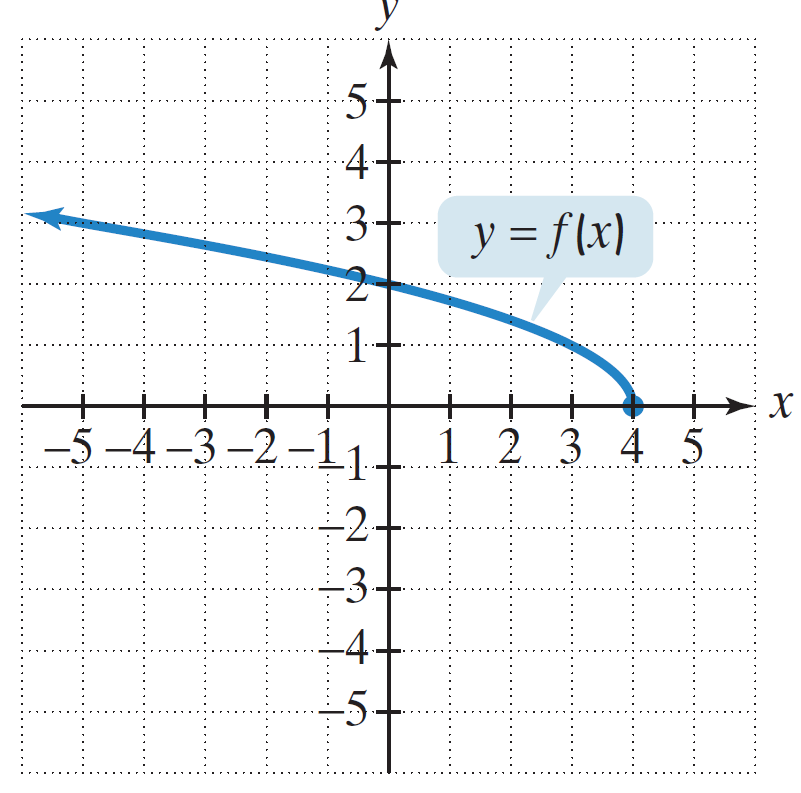
\includegraphics[scale=.3]{images/dom_rang_01}
\end{minipage}%
\begin{minipage}{.5\textwidth}
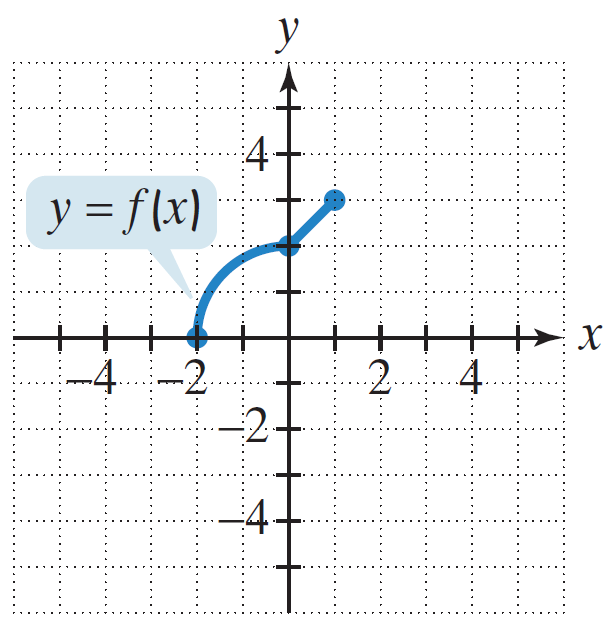
\includegraphics[scale=.4]{images/dom_rang_02}
\end{minipage}%
\vspace{1in}

\begin{minipage}{.5\textwidth}
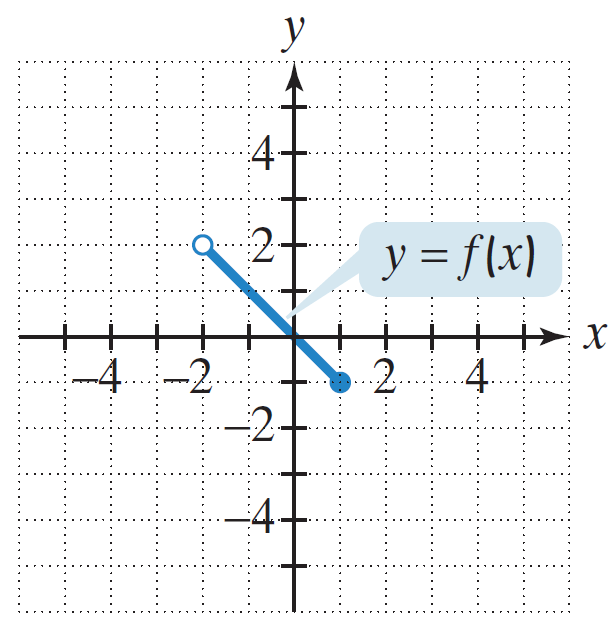
\includegraphics[scale=.4]{images/dom_rang_03}
\end{minipage}%
\begin{minipage}{.5\textwidth}
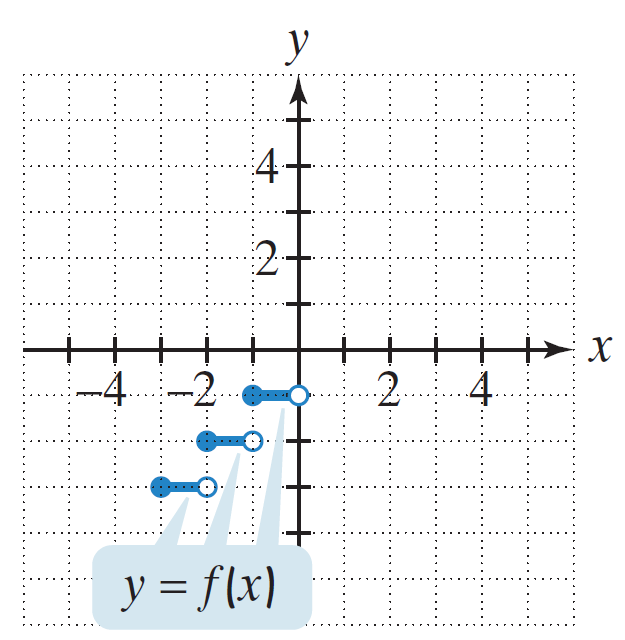
\includegraphics[scale=.4]{images/dom_rang_04}
\end{minipage}%
\vspace{1in}

\end{example}

\end{document}